\section{Durchführung}
\label{sec:Durchführung}

\begin{figure}[H]
  \centering
  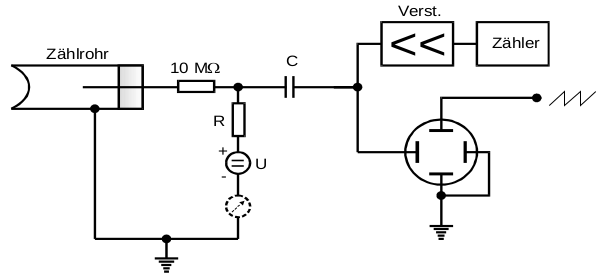
\includegraphics[height=6cm]{aufbau.png}
  \caption{Aufbau der Messapparatur.}
  \cite{skript}
  \label{fig:aufbau}
\end{figure}
Zur Durchführung der Messungen wird der Aufbau aus Abbildung \ref{fig:aufbau}
verwendet. Zunächst wird die Charakteristik der Zählrohrs aufgenommen, dazu
wird eine $\beta$-Quelle vor dem Zählrohr platziert. Nun wird die
Zählrate in Abhängigkeit der Spannung $U$ gemessen, dabei wird diese
von 300-700\;V variiert. Es ist zu beachten 700\;V nicht zu überschreiten, das
sonst der Bereich der selbstständigen Gasentladung erreicht wird und das
Zählrohr zerstört wird. Außerdem wird die Stromstärke am Zählrohr abgelesen.\\
Die Nachentladung wird nur qualitativ überprüft, indem sie auf dem
Oszilloskop sichtbar gemacht wird.
Um die Totzeit zu messen gibt es zwei Varianten.\\
1) Die Totzeit sowie die Erholungszeit werden auf dem Oszilloskop sichtbar gemacht.\\
2) Zwei-Quellen-Methode: Die Zählrate zwei verschiedener Quellen wird
 sowohl einzeln als auch zusammen gemessen.
